\section{Computational intelligence}

\subsection{Introduction}

Definitions to start the course 
\begin{itemize}
    \item \textbf{Problem} \ra Task to be solved automatically (find the maximum number in a list)
    \item \textbf{Algorithm} \ra Process to solve a problem, set of precise and not ambiguous actions that all together will allow us to reach the solution
    \item \textbf{Program} \ra Translation of an algorithm into a programming language
\end{itemize}

Motivation

\begin{itemize}
    \item In classical computational methods we start from a problem, and we have a human being that imagines an algorithm (problem-solving, it's creative and informal). Then software engineers will put the ideas into a computer in order to get a program (implementation, it's automatic and not creative). 
    \item We need computational intelligence because traditional methods in many cases fail, usually on the first step. We can have many problems where imaging solutions or algorithms it's either impossible or very hard for human being to imagine a solution. This is the case of \textbf{complex problems}
\end{itemize}


Some examples of complex problems
\begin{itemize}
    \item Categorization of clients
    \item Face recognition
    \item Find a new drug to cure a disease
    \item Driving a robot in a 3-D space 
\end{itemize}

Our idea is to give computers or informatic systems the ability to learn autonomously how to solve a problem. We define \textbf{learning} as improving something by means of experience. Those computers can also understand that the generated solution in not good enough, and so they should understand a better way to find the optimal solution. 

\vspace{10pt}

One of the most famous ways to improve those computers are bio-inspired algorithms. Like the \textbf{neural networks} (took inspiration from the brain), \textbf{evolutionary computation} (theory of evolution from Darwin, considering evolution as a sort of learning) where we have genetic algorithms, differential evolution or genetic programming, \textbf{swarm intelligence based algorithms} (system of animals are better at solve problems with respect to singular entities) like particle swarm optimization, \textbf{fuzzy systems} and \textbf{local search} like hill climbing simulated annealing.  

\vspace{10pt}

One category of complex problems are the so-called optimization problems. Even though they are complex they are easy to comprehend and to analyze.

Informally solving an optimization problem means to find the best solution(s) in a typically huge set of possible alternative solutions. We are able to find if something is a solution and to evaluate the quality of the solution with respect to the others. More formally an optimization problem is a pair of objects S and f where
\begin{itemize}
    \item S \ra set of all existing solutions (search space)
    \item f \ra function that evaluates the solutions (fitness or cost or quality function)
\end{itemize}

An optimization problem can be:

\[
\textbf{Maximization:} \quad \text{find } x^\ast \in S \text{ such that } 
f(x^\ast) \geq f(y) \quad \forall y \in S.
\]

\[
\textbf{Minimization:} \quad \text{find } x^\ast \in S \text{ such that } 
f(x^\ast) \leq f(y) \quad \forall y \in S.
\]

To solve this kind of problems we can use an optimization algorithm, a machine that is able to output multiple solutions (iterative machine). 

\vspace{10pt}

\textbf{No free lunch theorem} \ra the average performance of all optimization algorithms calculated on all existing optimization problems is the same. We care about the probability of finding the best solution and the time to reach it. We can't have one algorithm for every problem then we need to find a solution for every problem.


\subsection{Optimization algorithms}

\textbf{Optimization problem} \ra a pair (S, f) where

\begin{itemize}
    \item S is the set of all solutions (search space)
    \item f is the function (fitness function) where f : S \ra \begin{math}
        \mathbb{R} 
    \end{math}
\end{itemize}

An optimization problem can be:

\[
\textbf{Maximization:} \quad \text{find } x^\ast \in S \text{ such that } 
f(x^\ast) \geq f(y) \quad \forall y \in S.
\]

\[
\textbf{Minimization:} \quad \text{find } x^\ast \in S \text{ such that } 
f(x^\ast) \leq f(y) \quad \forall y \in S.
\]

x can be either a global optimum or a local one, we want to find the global(s) optima.

\vspace{10pt}

To find the solution we will use some optimization algorithm, by definition an optimization algorithm is an iterative method that at the end of each iteration returns a solution \begin{math}
    \in 
\end{math} S. One of the usual algorithm is \textbf{Random search}. 

As already seen we have the no free lunch theorem that stops us from finding a perfect solution. 

\vspace{10pt}
\textbf{No Free Lunch Theorem} \ra 
Let $A_1$ and $A_2$ be two optimization algorithms. 
When performance is averaged uniformly over all possible objective functions, 
$A_1$ and $A_2$ have identical expected performance.

\vspace{10pt}

The consequences of this theorem are that
\begin{enumerate}
    \item It is impossible to have an algorithm that is better than all the others and on all possible problems (no super algorithm can exist).
    \item Given a problem it can't exist an automatic method to find the best algorithm. Then we need to test, experiment and use our prior knowledge.
\end{enumerate}

\vspace{10pt}

Now we will see some algorithms. We start with \textbf{Hill climbing}. Before anything we need to clarify that we can't find every possible solution, so we need to use certain starting points.

\vspace{10pt}

\textbf{Neighborhood.}
Let $N : S \to 2^S$ be a neighborhood function that maps a solution 
$x \in S$ to a set of neighboring solutions $N(x) \subseteq S$.

Starting from an initial solution $x_0$ (typically chosen at random), 
the objective function is evaluated over $N(x_k)$, and the best 
neighbor is selected:
\[
x_{k+1} = \arg\min_{y \in N(x_k)} f(y)
\]
(for a minimization problem).

This process is repeated iteratively until a stopping criterion is met.

\vspace{10pt}

\textbf{Example}

\vspace{10pt}

\begin{itemize}
    \item S = {students in the room}
    \item f = student number 
    \item Maximization problem
    \item Neighborhood = the students around the selected student
\end{itemize}

\textbf{Local optimum} \ra given an optimization problem (S, f) a local optimum is a solution x such that $\forall y \in N(x), f(x)$ is better than $f(y)$. By definition hill climbing will return a local optimum with no guarantee that it will also be global. We can find the global optimum by expanding the radius or by trying more initialization

\vspace{10pt}

In pseudocode (general case)

\begin{enumerate}
    \item Initialize the current solution $x$ (typically at random).
    \item Repeat
    \begin{enumerate}[label=\theenumi.\arabic*]
        \item Generate a neighbor $y$ of $x$.
        \item If $f(y)$ is better than or equal to $f(x)$, set $x := y$.
    \end{enumerate}
    Until for all neighbors $y$ of $x$, $f(y)$ is worse than $f(x)$.
    \item Return $x$.
\end{enumerate}

In strict hill climbing we change the point only if the fitness is strictly better than the previous. With this setting we can have an infinite iteration between 2 equal points. We can set a timeout if we see the same points n times. 

Taboo search can help the search by using memory, avoid the already checked points. 

\vspace{10pt}

\textbf{Example}

\vspace{10pt}

\begin{itemize}
    \item $S = \{ i \in \mathbb{N} : 0 \le i \le 15 \}$
    \item  f(i) number of 1s in the binary code of i
    \item Maximization
    \item Neighborhood = i and j $\iff$ |i - j| = 1
\end{itemize}


We produce a plot

\begin{itemize}
    \item X \ra all solutions produced ordered by their neighborhood
    \item Y \ra all the fitness values
\end{itemize}

\begin{figure}[h!]
\centering
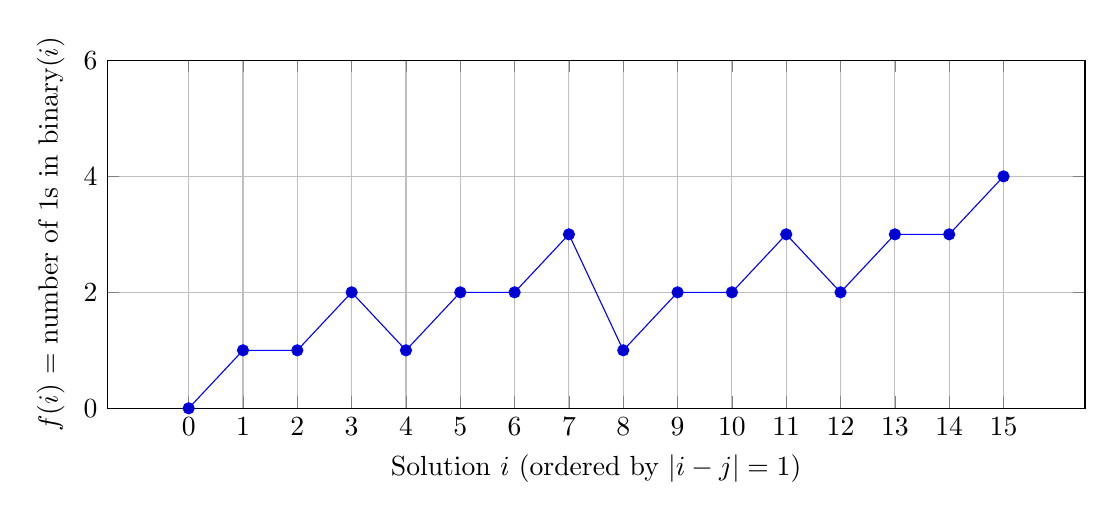
\begin{tikzpicture}
\begin{axis}[
    width=14cm,
    height=6cm,
    xlabel={Solution $i$ (ordered by $|i-j|=1$)},
    ylabel={$f(i)$ = number of 1s in binary$(i)$},
    xtick={0,...,15},
    ymin=0,
    ymax=6,
    grid=major
]

\addplot+[mark=*] coordinates {
(0,0)
(1,1)
(2,1)
(3,2)
(4,1)
(5,2)
(6,2)
(7,3)
(8,1)
(9,2)
(10,2)
(11,3)
(12,2)
(13,3)
(14,3)
(15,4)
};

\end{axis}
\end{tikzpicture}
\caption{Fitness landscape for $S=\{0,\dots,15\}$ with neighborhood $|i-j|=1$.}
\end{figure}

With the fitness landscape we can find the difficulty of the problem. A very smooth one is usually of a simple problem while a very oscillating one will be probably more difficult.


\subsection{Fitness landscape}

In the last class we saw what is a fitness landscape. The plot in the 2-D setting is obtained by plotting on the axis

\begin{itemize}
    \item Horizontal \ra All individual in the search space sorted according to the neighborhood
    \item Vertical \ra the fitness
\end{itemize}

Given an optimization problem (S, f) and a neighborhood N, a solution $x \in S$ is called a local optimum if $\forall y \in N(x)$ f(y) is worse than f(x). By construction hill climbing will return a local optimum with no guarantee that it will also be a global optimum.

\vspace{10pt} 

The fitness landscape gives a visual idea of how easy/hard is for an algorithm to solve the problem
\begin{itemize}
    \item Smooth \ra easy
    \item Rugged \ra hard
\end{itemize}

But in practice we can't draw the landscape because the search space is humongous, and the neighborhood is usually multidimensional.

\vspace{10pt}

Example
\begin{itemize}
    \item $S = \{ i \in \mathbb{N} | 0 \le i \le 15 \}$
    \item f(i) = $i^2$
    \item N = The solutions x and y are neighbors $\iff |x-y| = 1$
    \item Maximization
\end{itemize}

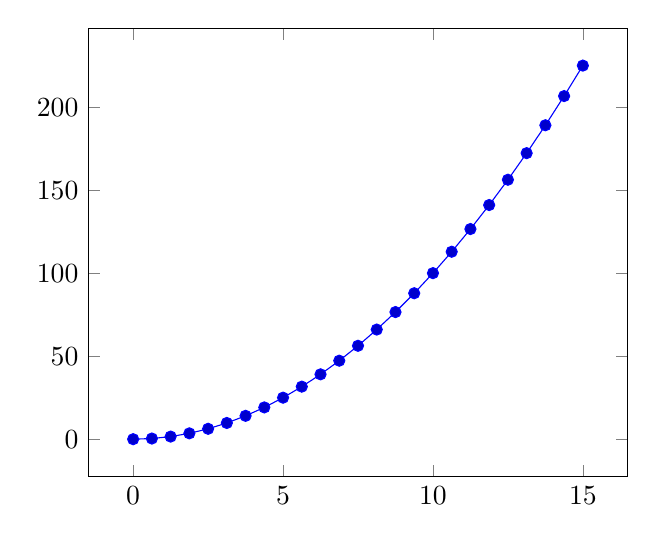
\begin{tikzpicture}
\begin{axis}[domain=0:15]
\addplot {x^2};
\end{axis}
\end{tikzpicture}

Here hill climbing will arrive at the global optimum.

\vspace{10pt}

If we want to look for the number of 1 in the binary code of i we can encounter problems and stay stuck in a local optimum without being able to find the global one. 
\vspace{10pt}

The definition of neighborhood is not fixed, we can define it in 2 ways.

\begin{itemize}
    \item N(x) \ra \{ $y \in s | d(x,y) \le k \}$ \ra distance based
    \item N(x) \ra \{ $y \in s | y = op(x) \}$ \ra action based
\end{itemize}


\begin{center}
\textbf{Example}
\end{center}

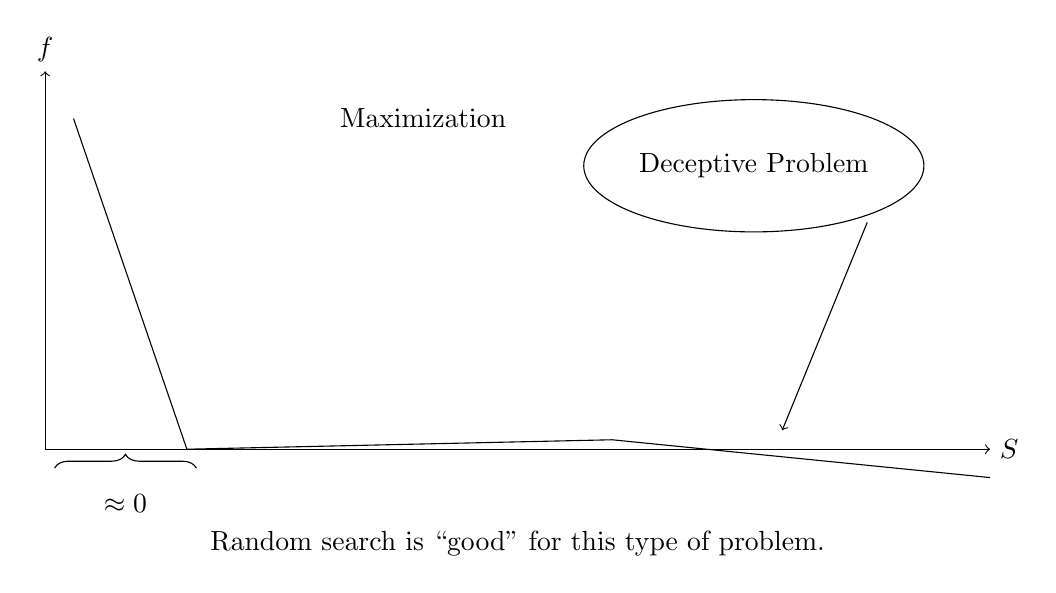
\begin{tikzpicture}[scale=1.2]

% axes
\draw[->] (0,0) -- (0,4) node[above] {$f$};
\draw[->] (0,0) -- (10,0) node[right] {$S$};

% deceptive peak near 0
\draw (0.3,3.5) -- (1.5,0);

% small mark around 0
\draw[decorate,decoration={brace,amplitude=5pt}]
(0.1,-0.2) -- (1.6,-0.2) node[midway,below=6pt] {$\approx 0$};

% almost flat line
\draw (1.5,0) -- (6,0.1) -- (8,-0.1) -- (10,-0.3);

% labels
\node at (4,3.5) {Maximization};

% deceptive problem bubble
\draw (7.5,3) ellipse (1.8 and 0.7);
\node at (7.5,3) {Deceptive Problem};

% arrow pointing to plateau
\draw[->] (8.7,2.4) -- (7.8,0.2);

% bottom text
\node at (5,-1) {Random search is ``good'' for this type of problem.};

\end{tikzpicture}

Hill climbing pros

\begin{itemize}
    \item Simple
    \item Efficient
    \item Versatile
\end{itemize}

Cons
\begin{itemize}
    \item Always stops on local optima
\end{itemize}

How to improve hill climbing

\begin{itemize}
    \item Parallel hill climbing
    \item Enlarge the neighborhood
    \item Give the possibility of worsening the fitness of the current solution (within a given probability)
\end{itemize}


\subsection{Annealing}

We now introduce the concept of annealing \ra an experiment aimed at finding the solid state of a material with the minimum level of energy.

\textbf{Metropolis algorithm}

\begin{enumerate}
    \item Consider the initial state of the material with energy $E_i$
    \item Alter the state to get a new energy $E_j$
    \item If $E_j \le E_i$ accept the new state and continue
    \item Else accept the state with probability $exp(-\frac{|E_i - E_j|}{K_B T})$
\end{enumerate}

Where 
\begin{itemize}
    \item T = Temperature
    \item $K_B$ = Boltzmann constant
\end{itemize}

\textbf{Simulated annealing}

\begin{itemize}
    \item Current solution = x
    \item Neighbor = y
\end{itemize}

\[
P(y) = \begin{cases}
    1 \text{ if f(y) better or equal than f(x)} \\
    exp(-\frac{|f(x) - f(y)}{C}) \text{ otherwise}
\end{cases}
\]

Where C is a control parameter

\subsection{Practical applications of Hill climbing}

Test case 1 \ra Given a set of possible investments (N), for each investment we know

\begin{itemize}
    \item Cost
    \item Estimated gain
\end{itemize}

We also know the budget of the client. What subset of the investments should our client do? 

Such that
\begin{itemize}
    \item The total cost is smaller or equal to the budget
    \item The profit is maximized
\end{itemize}


Using a numeric example

\begin{itemize}
    \item N = 10
    \item Costs = \{23, 31, 29, 44, 53, 38, 63, 85, 89, 82 \}
    \item Profits = \{92, 57, 49, 68, 60, 43, 67, 84, 87, 72 \}
    \item Budget = 165
\end{itemize}

\vspace{10pt}
Questions to answer
\begin{enumerate}
    \item What are the solutions ?
    \item How it is convenient to represent the solutions?
    \item What's the fitness?
    \item If the algorithm is neighborhood based, then what is the neighborhood?
\end{enumerate}

Golden rule \ra \textbf{DO NOT solve the problem}

Answers

\begin{enumerate}
    \item All the subsets of the set of investments
    \item As sequences of values, a string of bits of length N. The array will have a pair of  cost and profit. We use 0s and 1s to "1-hot encoding" them. 
    \item The sum for all the indexes where x is 1 of all the profits. $\sum\limits_{i:x[i]=1} p[i]$. We have a maximization problem. We only care about solutions that have a cost less than the budget. The fitness if this condition is not accepted we have -1 or 0 as fitness. Another way to define a non-good fitness is to use the negative sum of the costs such that the distance ourselves as much as possible from a bad solution. 
    \item The neighborhood is obtained here using the bit flip operator. 
\end{enumerate}


\vspace{10pt}

Test case 2 \ra Travel-sale-person: given N cities for which we know all the pairwise distances between themselves. Give one of these cities there is one specific one that is called home. We want the cyclic path that starts from home, visits all the cities once and only once and terminates at home using the shortest possible path.

\vspace{10pt}

We start from a matrix 

\begin{itemize}
    \item N = 5 \ra the matrix is 5x5
    \item Inside the matrix we have the costs/distances
\end{itemize}

Answers 

\begin{enumerate}
    \item Solutions \ra All cyclic paths starting and finishing in home and visiting all cities once. 
    \item Representation \ra An ordered string of the cities
    \item Fitness \ra the sum of the distances in the string
    \item Neighborhood \ra We can use a swapping operator
\end{enumerate}



\subsection{Simulated annealing}

Simulated annealing is similar to hill climbing, but we add the concept of probability. This can lead to a worse fitness. The idea is that we can explore more possible solutions and obtain a better optimum. But we can also miss some of those. Sometimes can be convenient that our current solution is a random neighbor.

\vspace{10pt}

We can start by defining our current solution $x$ and our candidate neighbor $y$.

The probability $P(y)$ is defined as:

\[
P(y) = 
\begin{cases} 
    1 & \text{if } f(y) \leq f(x) \\
    \exp\left(-\frac{|f(x) - f(y)|}{C}\right) & \text{otherwise}
\end{cases}
\]

Where $C$ is a control parameter $C > 0$.

\vspace{10pt}

Afterward, we look for a random number in the interval $[0, 1]$ and if this number is $< P(y)$, we accept the move.

We start with a large $C$, and we decrease it during the algorithm. $C$ will tend to $0$ without reaching it, following the cooling schedule:

\[
C = \frac{C}{h}
\]

Simulated annealing follows the following structure

\begin{enumerate}
    \item Initialize the current solution x (typically at random)
    \item Initialize C and L
    \item Repeat the following until termination
    \begin{itemize}
        \item Repeat L times
        \begin{itemize}
            \item Create a random neighbor x of y
            \item Accept or not y with a certain probability 
        \end{itemize}
    \item Update C (not mandatory update L)
    
    \end{itemize}
    \item Return x (or the best solution so far)
\end{enumerate}

We terminate when we have found a certain condition that can be either a good enough solution or we have run a prefixed maximum number of iterations of the external loop.

\vspace{10pt}

\textbf{Example}

\begin{itemize}
    \item S = {i $\in \mathbb{N} | 0 \le i \le 15$ }
    \item $\forall i \in S, f(i) = $ number of 1s in the binary code of i
    \item Maximization
    \item Neighborhood \ra x and y are neighbors $\iff |x-y|=1$
\end{itemize}

\noindent
\textbf{Step 1: Initialization} \\
$x = 5$ (random initialization) $\rightarrow bin(5) = 101$ \\
$f(x) = 2$ \\
$N(x) = \{4, 6\}$ \\
\textbf{Assume} $y = 6$ (random neighbor) $\rightarrow bin(6) = 110$ \\
$f(y) = 2$ \\
Since $f(y) \leq f(x)$, we accept the move: $x = 6$.

\vspace{10pt}

\noindent
\textbf{Step 2: Iteration} \\
$x = 6$ \\
$N(x) = \{5, 7\}$ \\
\textbf{Assume} $y = 7$ (random neighbor) $\rightarrow bin(7) = 111$ \\
$f(y) = 3$ \\
Since $f(y) > f(x)$, we calculate the acceptance probability.

\vspace{10pt}

\noindent
\textbf{Step 3: Probability Calculation} \\
Assume in this phase the control parameter is $C = 1$. \\
Current state: $f(x) = 3$ \\
Candidate neighbor: $f(y) = 1$

\[
P(acc \ y) = \exp\left( -\frac{|3 - 1|}{1} \right) = e^{-2} \simeq 0.13
\]

\vspace{5pt}
\noindent
This value represents a \textit{``large'' probability} for this phase of the algorithm.

\vspace{10pt}

\textbf{Theorem of asymptotic convergence of simulated annealing}

\vspace{10pt}

Given an optimization problem (S, f) and an appropriate neighborhood, if we decrease C so that it tends to 0 (without reaching it):

\noindent
As $t \rightarrow \infty$ and $C \rightarrow 0$, we analyze the convergence:

\[
\lim_{C \to 0} q_i(C) = \frac{1}{|S_{opt}|} \cdot g(i)
\]

\noindent
\textbf{Where:}
\begin{itemize}
    \item $q_i(C)$ is the probability that Simulated Annealing (SA) will stabilize on solution $i$ with control parameter $C$.
    \item $S_{opt}$ is the set of global optima.
    \item $g(i)$ is an indicator function defined as:
\end{itemize}

\[
g(i) = 
\begin{cases} 
    1 & \text{if } i \in S_{opt} \\
    0 & \text{otherwise}
\end{cases}
\]

\vspace{10pt}
\noindent
This limit shows that as the temperature $C$ approaches zero, the probability of being in a state $i$ becomes uniform over the set of global optimal solutions and zero elsewhere. To be sure to find a global optimum we should execute the process a very large number of times.

\vspace{10pt}

The parameters L and C are respectively Large and slow (decreasing)

\subsection{Genetic algorithms}

Genetic algorithms share similarities with simulated annealing

\begin{itemize}
    \item Both are optimization algorithms
    \item Both allow to look for good solutions without an exhaustive analysis of the search space
    \item Both start from random solutions and improve their quality iteratively
\end{itemize} 

The differences on the other hand are

\begin{itemize}
    \item The solutions (individuals) that are considered at a time are more than 1 (population)
    \item Inspired by the theory of evolution of Charles Darwin
    \item Individuals must be represented by strings of constant length
\end{itemize}


The theory of evolution has the following key elements
\begin{itemize}
    \item Reproduction
    \item Ability of adaptation
    \item Inheritance
    \item Variation
    \item Competition
\end{itemize}

\begin{figure}[h]
    \centering
    \begin{tikzpicture}[
        node distance=2cm and 3cm,
        block/.style={rectangle, draw, minimum width=3cm, minimum height=2cm, align=center, thick},
        arrow/.style={-Stealth, thick}
    ]

    % Nodi (I box del tuo disegno)
    \node[block] (P) {Pop. $P$ \\ of $N$ individuals};
    \node[block, right=of P] (P1) {Pop. $P'$ \\ of $N$ individ.};
    \node[block, below right=1cm and 0.5cm of P] (P2) {Pop. $P''$ \\ of $N$ indiv.};

    % Etichette sopra i box
    \node[above=0.1cm of P1, font=\small] {POP. OF PARENTS};
    \node[below=0.1cm of P2, font=\small] {POP. OF OFFSPRING};

    % Frecce con etichette
    \draw[arrow] (P) -- node[above] {SELECTION} node[below] {PROCESS} (P1);
    
    \draw[arrow] (P1.south) .. controls +(0,-2) and +(2,0) .. 
        node[right, align=left, xshift=0.5cm] {REPRODUCTION \\ WITH VARIATION \\ (CROSSOVER AND \\ MUTATION)} (P2.east);
        
    \draw[arrow] (P2.west) .. controls +(-2,0) and +(0,-2) .. 
        node[left, xshift=-0.5cm] {$P := P''$} (P.south);

    \end{tikzpicture}
    \caption{Genetic Algorithms Cycle}
\end{figure}

\noindent
The \textbf{Selection Process} maps the initial population $P$ to the intermediate population $P'$ (parents):

\vspace{10pt}

\begin{center}
    Population $P$ \hspace{2cm} Population $P'$ \\
    \vspace{5pt}
    \fbox{
        \begin{tabular}{cc}
            A & B \\
            C & D
        \end{tabular}
    }
    \hspace{1.5cm} $\xrightarrow{\text{Selection}}$ \hspace{1.5cm}
    \fbox{
        \begin{tabular}{cc}
            A & A \\
            A & C
        \end{tabular}
    }
\end{center}

\vspace{10pt}

\noindent
In this example, individual \textbf{A} is selected three times due to its high fitness, \textbf{C} is selected once, while \textbf{B} and \textbf{D} are discarded.

\vspace{10pt}

The selection process is made of iterations of N independent executions of a selection algorithm. The selection algorithm chooses 1 solution from a population P.

The algorithm has the following general principles

\begin{enumerate}
    \item It's probabilistic
    \item Given any pair of independent A and B in P if f(A) is better than f(B) then A has a bigger probability than B of being selected
    \item No individual in P has a probability equal to 0 of being chosen
\end{enumerate}

\noindent
\textbf{Fitness Proportionate (Roulette Wheel) Selection} \\
Given $N$ individuals in population $P = \{1, 2, \dots, N\}$, for each $i = 1, 2, \dots, N$ we define the probability of selection as:

\[
P(sel \ i) = \frac{f_i}{\sum_{j \in P} f_j}
\]

\vspace{10pt}

\noindent
\textbf{Mechanism ($N = 4$):} \\
This method acts like a roulette wheel where the area of each slice $i$ is proportional to its fitness $f_i$. 
Individuals with higher fitness occupy a larger portion of the wheel, increasing their chances of being selected when the wheel is "spun" (represented by a random number $U \in [0, 1]$).

\begin{itemize}
    \item $i_1, i_2, i_3, i_4$: Individuals in the population.
    \item $U$: Random pointer used to select the individual.
\end{itemize}

Other ways that can be used are \textbf{Ranking} and \textbf{Tournament} selection.




\subsection{Again Genetic algorithms}

We forgor something about simulated annealing. The theorem that we talked about miss something.

Basically we can only use simulated annealing in an appropriate algorithm, but we didn't define what we meant by appropriate. 

\vspace{10pt}

From the part of asymptotic convergence. We must have a certain property \ra given any pair of solutions x and y it must be possible to build a sequence of solutions $a_1, a_2,..., a_n$ such that $\forall i = 1,2,3,...,n-1, a_i \text{ and } a_{i+1} $are neighbors. So $a_1=x$ and $a_n=y$. We say that the neighborhood is completely connected. 



\vspace{10pt}

Now going back to genetic algorithms.

We start with a population P of N individuals. N is a hyperparameter. We modify the population with two steps.
\begin{itemize}
    \item Selection phase \ra We have a population P' of N individuals
    \item Reproduction with Variation phase \ra We have a population P'' of N individuals
\end{itemize}

The new current population will be P'' and we repeat the two phases until we reach a stopping criterion, and we select as solution the best individual in the final P. 

We create new individuals (offspring) via means of crossover and mutation.

\vspace{10pt}

The idea behind this algorithm comes from the Darwinian ideas of adaptation, competition, reproductions, inheritance and variation. The first two are for the first phase, while the other 3 for the second one. The selection phase is an iteration of N independent executions of a selection algorithm where the objective is to choose one solution from a population of N solutions. 

\vspace{10pt}

Is important that the selection algorithm is probabilistic since we want to have different solutions every time. The probability of selecting a solution must be based on fitness. All individuals must have a non-zero probability of being selected. 

\vspace{10pt}

In this course we will talk about 3 main selection algorithms

\subsubsection{Fitness proportionate selection}

Also known as roulette wheel. We have a population of N individuals called 1, 2,..., n. For each i in 1, 2,..., n we have that the probability of selecting i we have $P(i) = \frac{f(i)}{\sum_{j \in P} f(j)}$. This is a maximization only algorithm, for minimization we can do 1 divided by fitness but if we have 0 fitness we use to add a constant to every possible value. 

\vspace{10pt}

The general take out concept is to adapt our solutions to every case. 


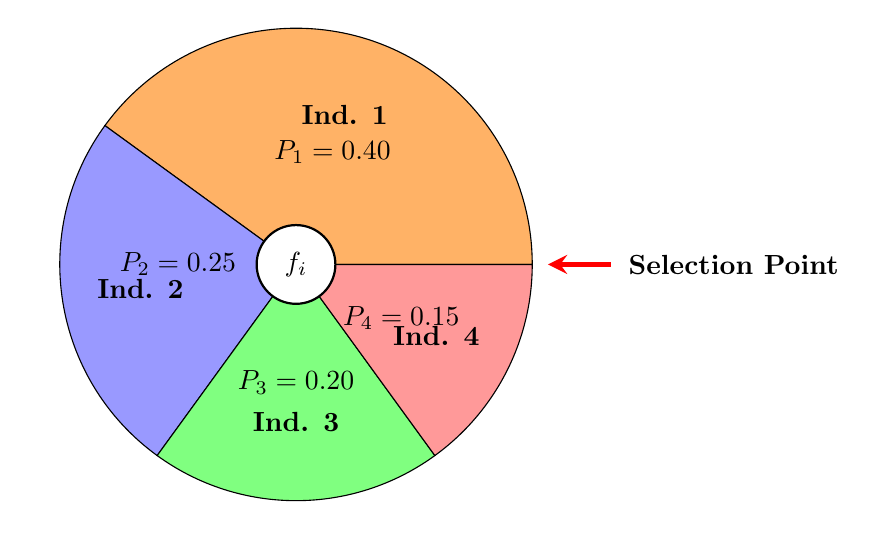
\begin{tikzpicture}
    % Definizione dei colori per i diversi individui
    \def\colorA{orange!60}
    \def\colorB{blue!40}
    \def\colorC{green!50}
    \def\colorD{red!40}

    % Disegno delle fette (angoli calcolati in base alla fitness)
    % Individuo 1 (40% -> 144 gradi)
    \filldraw[fill=\colorA, draw=black] (0,0) -- (0:3) arc (0:144:3) -- cycle;
    % Individuo 2 (25% -> 90 gradi)
    \filldraw[fill=\colorB, draw=black] (0,0) -- (144:3) arc (144:234:3) -- cycle;
    % Individuo 3 (20% -> 72 gradi)
    \filldraw[fill=\colorC, draw=black] (0,0) -- (234:3) arc (234:306:3) -- cycle;
    % Individuo 4 (15% -> 54 gradi)
    \filldraw[fill=\colorD, draw=black] (0,0) -- (306:3) arc (306:360:3) -- cycle;

    % Etichette centrali (Individui e Probabilità)
    \node at (72:2) {\textbf{Ind. 1}};
    \node at (72:1.5) {$P_1 = 0.40$};
    
    \node at (189:2) {\textbf{Ind. 2}};
    \node at (180:1.5) {$P_2 = 0.25$};
    
    \node at (270:2) {\textbf{Ind. 3}};
    \node at (270:1.5) {$P_3 = 0.20$};
    
    \node at (333:2) {\textbf{Ind. 4}};
    \node at (333:1.5) {$P_4 = 0.15$};

    % Disegno della freccia di selezione (Pointer)
    \draw[line width=2pt, -stealth, red] (4,0) -- (3.2,0);
    \node[anchor=west] at (4.1,0) {\textbf{Selection Point}};

    % Titolo o decorazione centrale
    \draw[fill=white, draw=black, thick] (0,0) circle (0.5);
    \node at (0,0) {$f_i$};

\end{tikzpicture}

\subsubsection{Ranking selection}

We follow this procedure

\begin{enumerate}
    \item Sort the individuals from the worst to the best based on fitness. 
    \item We calculate the probability selection based on the indexes. So $P(i) = \frac{\text{index}}{\sum \text{indexes}} $
\end{enumerate}

This algorithm is not sensitive to fitness differences, we don't care about how much a certain individual is better than another one. We can generalize this algorithm by changing the function (now is linear) to have a logarithm, an exponential and so on. This can change the selection pressure. 


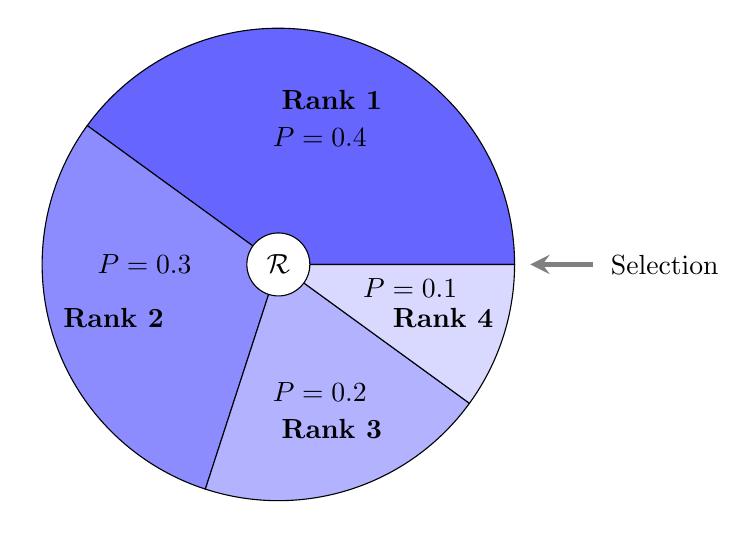
\begin{tikzpicture}
    % Definizione colori
    \def\colorRankOne{blue!60}
    \def\colorRankTwo{blue!45}
    \def\colorRankThree{blue!30}
    \def\colorRankFour{blue!15}

    % Rappresentazione a "gradini" o Ruota basata su Rank
    % Supponiamo 4 individui. Somma ranghi = 1+2+3+4 = 10.
    % Spazi: 4/10 (144°), 3/10 (108°), 2/10 (72°), 1/10 (36°)

    % Rank 1 (Il migliore) - 144 gradi
    \filldraw[fill=\colorRankOne, draw=black] (0,0) -- (0:3) arc (0:144:3) -- cycle;
    % Rank 2 - 108 gradi
    \filldraw[fill=\colorRankTwo, draw=black] (0,0) -- (144:3) arc (144:252:3) -- cycle;
    % Rank 3 - 72 gradi
    \filldraw[fill=\colorRankThree, draw=black] (0,0) -- (252:3) arc (252:324:3) -- cycle;
    % Rank 4 (Il peggiore) - 36 gradi
    \filldraw[fill=\colorRankFour, draw=black] (0,0) -- (324:3) arc (324:360:3) -- cycle;

    % Etichette
    \node at (72:2.2) {\textbf{Rank 1}};
    \node at (72:1.7) {$P = 0.4$};
    
    \node at (198:2.2) {\textbf{Rank 2}};
    \node at (180:1.7) {$P = 0.3$};
    
    \node at (288:2.2) {\textbf{Rank 3}};
    \node at (288:1.7) {$P = 0.2$};
    
    \node at (342:2.2) {\textbf{Rank 4}};
    \node at (350:1.7) {$P = 0.1$};

    % Pointer
    \draw[line width=2pt, -stealth, gray] (4,0) -- (3.2,0);
    \node[anchor=west] at (4.1,0) {Selection};

    % Centro
    \draw[fill=white] (0,0) circle (0.4);
    \node at (0,0) {$\mathcal{R}$};

\end{tikzpicture}

\subsubsection{Tournament selection}

We follow the following schema (To draw). 


This can be considered as both random and deterministic.

\begin{enumerate}
    \item It is possible (in some cases) to not evaluate all the possible individual's fitness.  
    \item We can change the selection pressure by changing the tournament size
\end{enumerate}


\begin{tikzpicture}[
    node distance=1.5cm,
    individual/.style={rectangle, draw, fill=gray!10, minimum width=2cm, minimum height=0.8cm, rounded corners},
    winner/.style={rectangle, draw=green!60!black, fill=green!10, minimum width=2cm, minimum height=0.8cm, rounded corners, line width=1.5pt},
    loser/.style={rectangle, draw=red!40, fill=red!5, minimum width=2cm, minimum height=0.8cm, rounded corners, dashed}
]

    % Titolo del Torneo
    \node[font=\Large\bfseries] at (2.5, 2) {Tournament Selection ($k=3$)};

    % Popolazione di sfondo (simbolica)
    \draw[dashed, gray] (-1,-4.5) rectangle (1.5, 0.5);
    \node[gray, rotate=90] at (-0.7,-2) {Population Pool};

    % Individui estratti per il torneo
    \node[individual] (ind1) at (3, 0) {Ind. A (Fit: 45)};
    \node[individual] (ind2) at (3, -1.5) {Ind. B (Fit: 82)};
    \node[individual] (ind3) at (3, -3) {Ind. C (Fit: 12)};

    % Frecce di estrazione dalla pool
    \draw[latex-, shorten <=2pt] (ind1.west) -- (1.5, 0);
    \draw[latex-, shorten <=2pt] (ind2.west) -- (1.5, -1.5);
    \draw[latex-, shorten <=2pt] (ind3.west) -- (1.5, -3);

    % Nodo del Vincitore
    \node[winner] (winner) at (10, -1.5) {Winner: Ind. B};

    % Frecce del confronto
    \draw[-Stealth, thick] (ind1.east) -- (winner.west) node[midway, above, sloped, font=\small] {loss};
    \draw[-Stealth, ultra thick, green!60!black] (ind2.east) -- (winner.west) node[midway, above, font=\small] {Best Fitness};
    \draw[-Stealth, thick] (ind3.east) -- (winner.west) node[midway, below, sloped, font=\small] {loss};

    % Nota sulla Pressione Selettiva
    \node[draw, fill=yellow!10, text width=4cm, font=\footnotesize, anchor=north] at (5, -4.5) {
        \textbf{Logic:} \\
        Pick $k$ individuals at random. \\
        The one with the highest fitness wins the tournament.
    };

\end{tikzpicture}


\subsection{Crossover and mutation}

Now we talk about the part about reproduction with variation. Selection depends only on phenotype while crossover and mutation only on genotype (DNA structure).


\subsubsection{Crossover}

We start by taking two solutions that are in P'. 

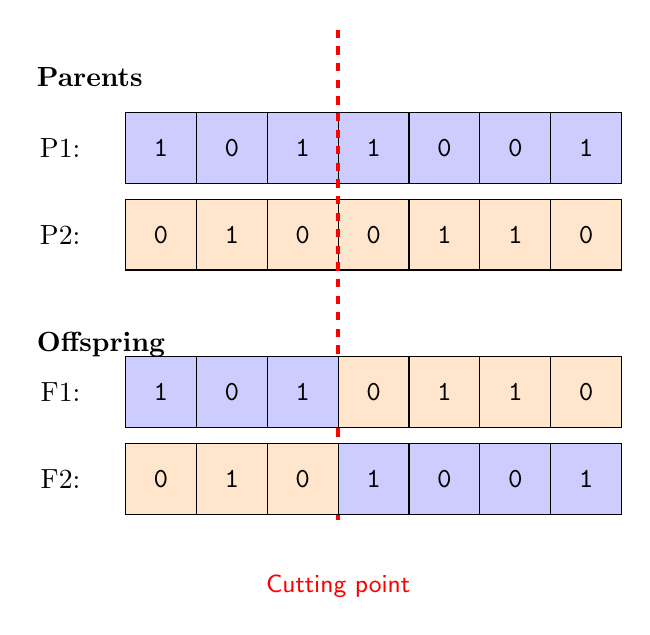
\begin{tikzpicture}
    \tikzset{bit/.style={rectangle, draw=black, minimum size=0.9cm, font=\ttfamily\bfseries}}
    \tikzset{highlight1/.style={fill=blue!20}}
    \tikzset{highlight2/.style={fill=orange!20}}

    % ── PARENTS ──────────────────────────────────────────
    \node[anchor=west, font=\bfseries] at (0, 2.2) {Parents};

    % Etichette riga
    \node[anchor=east] at (0.8, 1.3) {P1:};
    \node[anchor=east] at (0.8, 0.2) {P2:};

    % P1
    \foreach \val [count=\i] in {1,0,1,1,0,0,1} {
        \node[bit, highlight1] at (\i*0.9+0.8, 1.3) {\val};
    }

    % P2
    \foreach \val [count=\i] in {0,1,0,0,1,1,0} {
        \node[bit, highlight2] at (\i*0.9+0.8, 0.2) {\val};
    }

    % ── LINEA DI TAGLIO (tra 3° e 4° bit) ───────────────
    % Centro del 3° bit: x = 3*0.9+0.8 = 3.5
    % Centro del 4° bit: x = 4*0.9+0.8 = 4.4
    % Punto di taglio: (3.5+4.4)/2 = 3.95
    \draw[red, ultra thick, dashed] (3.95, 2.8) -- (3.95, -3.5);
    \node[below, font=\small\sffamily, text=red] at (3.95, -4.0) {Cutting point};

    % ── OFFSPRING ────────────────────────────────────────
    \node[anchor=west, font=\bfseries] at (0, -1.2) {Offspring};

    % Etichette riga
    \node[anchor=east] at (0.8, -1.8) {F1:};
    \node[anchor=east] at (0.8, -2.9) {F2:};

    % F1: primi 3 da P1 + ultimi 4 da P2
    \foreach \val [count=\i] in {1,0,1} {
        \node[bit, highlight1] at (\i*0.9+0.8, -1.8) {\val};
    }
    \foreach \val [count=\i] in {0,1,1,0} {
        \node[bit, highlight2] at (\i*0.9+3.5, -1.8) {\val};
    }

    % F2: primi 3 da P2 + ultimi 4 da P1
    \foreach \val [count=\i] in {0,1,0} {
        \node[bit, highlight2] at (\i*0.9+0.8, -2.9) {\val};
    }
    \foreach \val [count=\i] in {1,0,0,1} {
        \node[bit, highlight1] at (\i*0.9+3.5, -2.9) {\val};
    }

\end{tikzpicture}


This example is for 1-point crossover, but we can have multiple cutting points. 


\subsubsection{Mutation}

For each character we change it with a given probability of mutation (another hyperparameter)


\subsubsection{General function of genetic algorithms}

Here we have a pseudocode on the general idea of genetic algorithms

\begin{enumerate}
    \item Initialize a population P of N individuals (typically at random)
    

    \item Repeat until termination condition is reached:
    

    \begin{enumerate}
        \item Calculate the fitness of all the individuals in the population P (can be avoided in some cases, like tournament selection). This step is computationally costly
        \item We create an empty population P'
        \item Repeat P' has N individuals
        \begin{enumerate}
            \item We choose a genetic operator (crossover with probability $P_c$ or replication with probability $1-P_c$)
            \item Select 2 individuals from population P 
            \item Apply the operator to the individuals 
            \item Apply mutation to the individuals resulting from the previous step 
            \item Insert the individuals resulting from the previous point into P' 
        \end{enumerate}
        \item Replace P with P'
    \end{enumerate}
    \item Return the best individual in P in terms of fitness
\end{enumerate}



Some points

\begin{itemize}
    \item If N is odd:
    \begin{itemize}
        \item Select 1 individual mutated and insert it into P'
        \item One crossover event copies into P' only one offspring (typically the best in fitness)
    \end{itemize}
    \item Elitism is the unchanged copy of the best K individuals in P into P' (bypassing the selection-crossover-mutation pipeline), typically K=1
    \item We have to do something like P \ra selection \ra P' \ra crossover + mutation \ra P'' \ra P := P'' 
    \item Replication is the unchanged copy of the parents
    \item Termination condition is either
    \begin{itemize}
        \item A good enough solution is found, and we return it
        \item A maximum number of generation was performed
    \end{itemize}
\end{itemize}


\subsubsection{Hyperparameters of genetic algorithms}

\begin{itemize}
    \item String length \ra Given by the problem definition
    \item Population size (N) \ra The bigger, the better. We have an upper bound (true for every problem)
    \item Selection algorithm that we want to use \ra No free lunch holds, but tournament selection can be interesting to use (fast, and we can use the selection pressure). We can start with this and try the others. The tournament size should not be too big (2 can be good, and the minimum). 
    \item Crossover probability ($P_c$) \ra Should be close to 1
    \item Mutation probability ($P_m$) \ra Should be close to 0
    \item Maximum number of generations \ra The bigger, the better but with an upper bound like for N
    \item Elitism on or off  (and if on size of the elite and k) \ra Elitism should be used with K=1
\end{itemize}




\subsection{Why genetic algorithms work}

To answer we have to have another question \ra Will genetic algorithms lead to the discovery of a global optimum or an approximation of it?

To answer we have to have another question \ra How do genetic algorithms work?

To answer we have to have another question \ra What is the information that is maintained and processed in the population?

\vspace{10pt}

The hypothesis that we want to verify is that there are some syntactic features that give a boost to fitness. We would like to maintain these features through generations. To do this we would like to formalize a mechanism to identify structural similarities between individuals. We can call it \textbf{Schema} (set of individuals that have in common the fact of having the same characters in some positions). 

\vspace{10pt}
A schema can be represented using strings composed by all admissible characters + 1 special character (don't care symbol, here is *). For example in the binary case, a schema is a string built using characters coming from the set \{0, 1, *\}.

\vspace{10pt}
Example

\{*0000\} represents both \{00000\} and \{10000\}.

\vspace{10pt}

Hypothesis \ra implicitly genetic algorithms work on schemata. 

\vspace{10pt}

\begin{itemize}
    \item Order of a schema \ra The number of characters different from *, o(\{011*1**\}) = 4
    \item Length of a schema \ra The difference between the rightmost and leftmost positions that do not have an *, $\delta$(011*1**) = 5 - 1 = 4
\end{itemize}

Now we want to know what schemata will survive in the population over the evolution of a genetic algorithm. 

\vspace{10pt}

At generation t, m(H, t) is the number of individuals in the population that belong to the schema H. Given this we want to know what is m(H, t + 1). To solve this we need to know how selection, crossover and mutation change m(H, t). 

\vspace{10pt}

\subsubsection{Effect of selection on schemata}

We will study the case of fitness proportionate selection. 

$m(H, t +1 ) = m(H, t) n \frac{f(H)}{\sum_{j}^{}f_j}$

Where f(H) is the average fitness of the individuals in the population that belong to schema H. In the denominator we have the average probability of selecting an individual belonging to schema H. We apply selection n times.

\vspace{10pt}
\[
\begin{aligned}
&\text{AVG. FIT. OF INDIVS IN POP} = \tilde{f} = \frac{\sum_{j} f_j}{n} \\
&\frac{1}{\tilde{f}} = \frac{n}{\sum_{j} f_j} \\
&m(H, t+1) = m(H, t) \frac{f(H)}{\tilde{f}}
\end{aligned}\]


\vspace{10pt}

Schemata with an average fitness that is better than the average population fitness will increment the number of representatives and the others will decrement. 
At what speed? 
\[
\begin{aligned}
&\text{Assume } f(H) = \tilde{f} + c\tilde{f} \\
m(H, t+1) &= m(H, t) \frac{\tilde{f} + c\tilde{f}}{\tilde{f}} = m(H, t) \frac{\tilde{f}(1+c)}{\tilde{f}} \\
&= m(H, t)(1+c)
\end{aligned}
\]

\[
\begin{aligned}
m(H, 1) &= m(H, 0)(1+c) \\
m(H, 2) &= m(H, 1)(1+c) = m(H, 0)(1+c)^2 \\
m(H, 3) &= m(H, 2)(1+c) = m(H, 0)(1+c)^3 \\
&\vdots \\
m(H, t) &= m(H, 0)(1+c)^t
\end{aligned} \]

\bigskip

\noindent \text{The growth of the number of representatives}
\text{of schema } H \text{ in the population is exponential} \\
\text{with } t.

\subsubsection{Effect of crossover on schemata}

\textbf{EXAMPLE}

\[
\begin{aligned}
A &= 0 \ 1 \ 1 \ | \ 1 \ 0 \ 0 \ 0 \\
H_1 &= * \ 1 \ * \ | \ * \ * \ * \ 0 \\
H_2 &= * \ * \ * \ | \ 1 \ 0 \ * \ *
\end{aligned}
\]

\bigskip

\noindent \textbf{FOR ANY SCHEMA} \quad \( P_s(H) = 1 - \frac{\delta(H)}{L-1} \)

\bigskip

\[
\begin{aligned}
P_d(H_1) &= \frac{5}{6} = \frac{\delta(H_1)}{L-1} \\
P_s(H_1) &= 1 - \frac{5}{6} = \frac{1}{6} \implies 1 - \frac{\delta(H_1)}{L-1}
\end{aligned}
\]

\noindent \textbf{IN GENERAL}
\[
P_s(H) \geq 1 - p_c \frac{\delta(H)}{L-1}
\]

\vspace{1em}

\subsubsection{Combined effect of selection and crossover}
\[
m(H, t+1) \geq m(H, t) \frac{f(H)}{\tilde{f}} \left[ 1 - p_c \frac{\delta(H)}{L-1} \right]
\]

\vspace{1em}

\noindent \textbf{Schemata with:} \\
$-$ The average fitness is better the population average  \\
$-$ The small length will increment the number of representatives exponentially


\subsubsection{Effect of mutation}

\noindent \text{The probability that 1 bit will not be changed} = 1 - $p_m$

\vspace{1em}

\noindent \text{The probability of a schema surviving mutation} =
\[
\underbrace{(1 - p_m)(1 - p_m)(1 - p_m) \dots (1 - p_m)}_{o(H) \text{ times}}
\]

\vspace{1em}

\[
P_s(H) = (1 - p_m)^{o(H)} \quad \quad 
\begin{aligned}
&\text{if } p_m \ll 1, \text{ then} \\
&P_s(H) \approx 1 - o(H) p_m
\end{aligned}
\]

\noindent \textbf{Schema theorem}
\[
m(H, t+1) \geq m(H, t) \frac{f(H)}{\tilde{f}} \left[ 1 - p_c \frac{\delta(H)}{L-1} \right] \left[ 1 - o(H) p_m \right]
\]

\vspace{1.5em}

\noindent \text{We have schemata that:}
\begin{itemize}
    \item[$-$] \text{Have an average fitness better than population average}
    \item[$-$] \text{Are short (small} $\delta(H)$\text{)}
    \item[$-$] \text{Have a small order (small} $o(H)$\text{)}
\end{itemize}


\noindent \text{will increase the number of representatives exponentially}


\subsubsection{Building blocks' hypothesis}

This hypothesis tells us that maintaining the building blocks in the population and making them increment exponentially will
\begin{itemize}
    \item Maximize our chances of finding a global optimum
    \item Make the probability of finding a global optimum tend to 1 with time
\end{itemize}


\subsubsection{K-armed bandit problem}

This looks like something random but apparently is related to genetic algorithms.

\vspace{10pt}

Vanneschi just trashed Samuel in real time.

\vspace{10pt}


\begin{itemize}
    \item Given N slot machines
    \item Every slot machine j has a number of arms $K_j$
    \item We assume that we already played t times and for each of this t games we know 
    \begin{itemize}
        \item The slot machine in which we played 
        \item The result of the game (win or lose)
    \end{itemize}
    \item We want to find to which slot machine we should allocate our next attempts to maximize our probability of winning 
\end{itemize}

Given the slot machine j, we call $S_j$ the probability of winning using the slot machine j estimated using all the past t attempts. So $S_j = \frac{\text{Number of games where we used slot machine j and we won}}{\text{Total number of game}}$

\vspace{10pt}

Theorem time \ra If in the next game we allocate a number of attempts to slot j such that

\begin{itemize}
    \item $S_j $ > average ($S_j > \frac{\sum_{i}S_i}{N}$)
    \item j has a small number of arms
\end{itemize}

Then \begin{itemize}
    \item We maximize our probability of winning
    \item The probability of winning tends to 1 with the number of attempts tending to infinity
\end{itemize}

The consequence is the theorem of asymptotic convergence of genetic algorithms.

Let i(t) be the best individual in the population at generation t and $S_o$ be the best set of global optima. Then \[\lim_{t\ra \infty} P(i(t) \in S_o) = 1\]

\subsection{Problems with genetic algorithms}

The main drawbacks of standard genetic algorithms are

\begin{enumerate}
    \item Premature convergence \ra also known as loss of diversity. For any possible problem our algorithm will produce individuals that are similar to each other. If they are not similar to the global optimum we might never reach it. 
    \item Position problem \ra typical of standard crossover. We risk splitting our good chromosomes if they are at different ends. 
    \item Unicity of the fitness
\end{enumerate}


We can solve them with the following methods

\subsubsection{Premature convergence}

We have ways to measure the diversity of our population and to see if we have this problem

\begin{itemize}
    \item Entropy \ra $\sum_{j = 1}^{N} F_j \log(F_j)$
    \item Variance \ra  $\frac{1}{n-1} \sum_{i=1}^{n} (x_i - \bar{x})^2$
\end{itemize}

Both can be measured on genotypic (within the individual) and phenotypic (fitness) dimensions. 

\begin{itemize}
    \item Phenotypic entropy \ra N is the number of different fitness values in the population and $F_j$ fraction of individuals with a specific fitness value in the population. For continuous fitness we usually define bins. 
    \item Genotypic entropy \ra N is the number of different genotypes while (strings) and $F_j$ the fraction of individuals with that genotype. 
    \item Phenotypic variance \ra n is the number of individuals in the population, $x_i$ is the fitness of individual i and $\bar{x}$ is the average fitness of the individuals in P. 
    \item Genotypic variance \ra n is the number of individuals in the population, $x_i$ (given a distance measure) is the distance of the individual i from the origin and $\bar{x}$ is the average distance to origin of the individuals in the population. 
\end{itemize}

As origin, we can choose any individual (usually a string of zeroes). These methods are just monitoring systems (not a way to solve the problems).


\vspace{10pt}

How to maintain diversity?

\vspace{10pt}

We can do
\begin{enumerate}
    \item Fitness sharing
    \item Restricted mating
\end{enumerate}

With fitness sharing we will give more fitness to individuals that are very diverse. Then similar individuals will be penalized. This approach doesn't change the representation of our individuals.

\vspace{10pt}

Restricted mating acts in the opposite way. 

\vspace{10pt}
\textbf{Fitness Sharing}
\vspace{10pt}

For all individuals i in the population:

\begin{itemize}
    \item Given a predefined distance measure calculate the distance from i to all the other individuals in the population
    \item Normalize all these distances in the interval [0, 1]
    \item Invert these distances (for instance calculating $S(i, j) = 1-d(i,j)$)
    \item Calculate the sharing coefficient the sharing coefficient of i \ra ($S(i) = \sum_{j}S(i,j)$)
    \item  Redefine the fitness as $f_{s}(i) = \frac{f(i)}{S(i)}$
\end{itemize}

We can do this given:

\begin{enumerate}
    \item A distance measure
    \item A normalization method
    \item A way to invert the distances
\end{enumerate}

\begin{center}
    \textbf{EXAMPLE}
\end{center}

\textbf{POPULATION} \\
$i_1: \quad 11111 \quad f(i_1) = 50$ \\
$i_2: \quad 01111 \quad f(i_2) = 40$ \\
$i_3: \quad 10111 \quad f(i_3) = 30$ \\
$i_4: \quad 00000 \quad f(i_4) = 10$

\vspace{1em}
\textbf{DISTANCE:} Hamming Distance \\
\textbf{NORMALIZATION:} $d_N = \frac{d}{L}$ \\
\textbf{INVERSION:} $1 - d_N$

\vspace{1em}
\textbf{MAXIMIZATION} \\
New fitness $i_4$:
\begin{align*}
    d(i_4, i_1) = 5 &\longrightarrow d_N = 1 \longrightarrow S = 0 \\
    d(i_4, i_2) = 4 &\longrightarrow d_N = \frac{4}{5} \longrightarrow S = \frac{1}{5} \\
    d(i_4, i_3) = 4 &\longrightarrow d_N = \frac{4}{5} \longrightarrow S = \frac{1}{5}
\end{align*}

\[ S(i_4) = 0 + \frac{1}{5} + \frac{1}{5} = \frac{2}{5} \]

The result is that we have implicit speciation.



\vspace{10pt}
\textbf{Restricted mating}
\vspace{10pt}

Starting from an arbitrary schema we divide it in two parts, template and functional. In the template we are basically coding what the individual will like from the mating point of view. We get that we can do cross over in a restricted way. 

The model are
\begin{itemize}
    \item Bi-directional match
    \item Uni-directional match
    \item Best partial match
\end{itemize}

\begin{center}
    \underline{\large \textbf{RESTRICTED MATING}}
\end{center}

\vspace{1em}

\begin{center}
    \begin{tabular}{r c l}
        & \textbf{$\langle$TEMPLATE$\rangle$} & \textbf{$\langle$FUNCTIONAL$\rangle$} \\
        $i_1:$ & $* \ 1 \ 0 \ *$ & $: \ 1 \ 0 \ 1 \ 0$ \\
        $i_2:$ & $* \ 0 \ 1 \ *$ & $: \ 1 \ 1 \ 0 \ 1$ \\
        $i_3:$ & $0 \ * \ * \ 0$ & $: \ 0 \ 0 \ 0 \ 0$ \\
    \end{tabular}
\end{center}

\subsubsection{Position problem}

Crossover tends to destroy good individuals if the good genomes are on different sides after the cut. If we want to save those genomes we would like to reorder the indexes, but we will have problems in doing it. Our objective is to take two parents with indexes in different orders and create children that have all indexes (once). We can do something called \textbf{Cycle Crossover}

\begin{center}
    \underline{\Large \textbf{CYCLE CROSSOVER}}
\end{center}

\vspace{1em}

\textbf{PARENTS} \\
\begin{tabular}{r cccccccccc}
    & 1 & 2 & 3 & 4 & 5 & 6 & 7 & 8 & 9 & 10 \\
    $P_1:$ & 1 & 1 & 0 & 0 & 0 & 1 & 1 & 0 & 0 & 1 \\
    $P_2:$ & 0 & 0 & 0 & 1 & 1 & 1 & 1 & 1 & 0 & 0 \\
\end{tabular}

\vspace{1em}
$\xrightarrow{\text{INVERSION}}$
\vspace{1em}

\begin{tabular}{r cccccccccc}
    Indices: & 9 & 8 & 2 & 1 & 7 & 4 & 5 & 10 & 6 & 3 \\
    Values $P_1$: & 0 & 0 & 1 & 1 & 1 & 0 & 0 & 1 & 1 & 0 \\
    Values $P_2$: & 0 & 1 & 0 & 0 & 1 & 1 & 1 & 0 & 1 & 0 \\
\end{tabular}

\vspace{1em}
$\xleftarrow{\text{REORDER}}$
\vspace{1em}

\textbf{OFFSPRING} \\
\begin{center}
    \fbox{
        \begin{minipage}{0.4\textwidth}
            1 0 0 0 1 1 1 1 0 0 \\
            0 1 0 1 0 1 1 0 0 1
        \end{minipage}
    }
\end{center}

\begin{itemize}
    \item \textbf{Step 1: Identifying a Cycle} 
    Start with the first gene of Parent 1 ($P_1$) and look at the gene in the same position in Parent 2 ($P_2$). You then find where that value from $P_2$ is located in $P_1$[cite: 1]. Repeat this process until you return to the starting value, which completes one "cycle"[cite: 1].
    
    \item \textbf{Step 2: Mapping (Inversion)} 
    In the example, the "Inversion" section shows the indices (1--10) rearranged to group them according to the cycles found[cite: 1]. For example, if indices 1, 4, and 5 form a cycle, they are analyzed together in this step[cite: 1].
    
    \item \textbf{Step 3: Selection and Swapping} 
    \begin{itemize}
        \item For the first cycle, the offspring inherit the genes directly from their respective parents in those positions[cite: 1].
        \item For the next cycle, the genes are "swapped": Offspring 1 gets genes from Parent 2, and Offspring 2 gets genes from Parent 1[cite: 1].
    \end{itemize}
    
    \item \textbf{Step 4: Reconstruction (Reorder)} 
    Finally, the genes are moved back into their original numerical positions (1 through 10)[cite: 1]. The values highlighted in \textbf{red} in the image represent the specific genes that were either swapped or kept as part of a cycle to create the final \textit{Offspring}[cite: 1].
\end{itemize}


Another way is to use \textbf{Partially matched crossover}

\begin{center}
    \underline{\Large \textbf{PARTIALLY MATCHED (MAPPED) CROSSOVER}}
\end{center}

\vspace{1em}

\textbf{PARENT 1} \\
\begin{tabular}{ccc|ccc|cccc}
    9 & 8 & 4 & \textbf{5} & \textbf{6} & \textbf{7} & 1 & 3 & 2 & 10 \\
    1 & 0 & 1 & \textbf{1} & \textbf{0} & \textbf{1} & 0 & 0 & 0 & 1 \\
\end{tabular}

\vspace{1em}

\textbf{PARENT 2} \\
\begin{tabular}{ccc|ccc|cccc}
    8 & 7 & 1 & \textbf{2} & \textbf{3} & \textbf{10} & 9 & 5 & 4 & 6 \\
    0 & 0 & 1 & \textbf{0} & \textbf{1} & \textbf{1} & 1 & 1 & 0 & 0 \\
\end{tabular}

\vspace{1em}
\hrule
\vspace{1em}

\textbf{OFFSPRING (Result)} \\
\begin{tabular}{ccc|ccc|cccc}
    9 & 8 & 4 & \textbf{2} & \textbf{3} & \textbf{10} & 1 & 6 & 5 & 7 \\
    1 & 0 & 1 & \textbf{0} & \textbf{1} & \textbf{1} & 0 & 0 & 1 & 1 \\
    \hline
    8 & 10 & 1 & \textbf{5} & \textbf{6} & \textbf{7} & 9 & 2 & 4 & 3 \\
    0 & 1 & 1 & \textbf{1} & \textbf{0} & \textbf{1} & 1 & 0 & 0 & 1 \\
\end{tabular}

\vspace{1em}

Sometimes we have to use the repair algorithm if some problems are coming.

We can have a new kind of mutation where we swap the character's order inside the window. 

% --- COPIA DA QUI ---
\begin{center}
\begin{tabular}{rrc}
    \textbf{Initial:} & $9 \quad 8 \quad \underline{\mathbf{4} \quad 5 \quad 6 \quad 7 \quad \mathbf{1}} \quad 3 \quad 2 \quad 10$ & \\[0.8em]
    & $\Downarrow$ & \\[0.8em]
    \textbf{mut1 (swap):} & $9 \quad 8 \quad \mathbf{1} \quad 5 \quad 6 \quad 7 \quad \mathbf{4} \quad 3 \quad 2 \quad 10$ & (swap) \\
    \textbf{mut2:} & $9 \quad 8 \quad \mathbf{1} \quad \mathbf{7} \quad \mathbf{6} \quad \mathbf{5} \quad \mathbf{4} \quad 3 \quad 2 \quad 10$ & 
\end{tabular}
\end{center}
% --- A QUI ---

\subsection{Multi-objective optimization}

We might have more than one fitness to optimize, then we need a way to optimize for all of them. 

% --- COPIA DA QUI ---
\begin{center}
\renewcommand{\arraystretch}{1.3}
\begin{tabular}{l @{\hspace{1cm}} l}
    \multicolumn{2}{l}{\textbf{MULTI-OBJECTIVE OPTIMIZATION (MULTI-FITNESS)}} \\[0.2em]
    \multicolumn{2}{l}{$\text{Fitness} = (\text{cost}, \text{avg. Numb. Of accidents})$} \\[1.5em]
    
    \textbf{Numeric Cases:} & \textbf{Global Pareto Optimal Set} = $\{A, B, C\}$ \\
    $A = (2, 10)$ & \small{(Set of the optima)} \\
    $B = (4, 6)$  & \\
    $C = (8, 4)$  & \textit{A, B, C are NON-DOMINATED:} \\
    $D = (9, 5)$  & There is no other global solution in the \\
    $E = (7, 8)$  & search space better in all criteria. \\
\end{tabular}

\vspace{1cm}

% GRAFICO IN PURO LATEX
\setlength{\unitlength}{4.5mm} % Scala del grafico leggermente aumentata
\begin{picture}(14,13)(-2,-1)
    % Assi cartesiani
    \put(0,0){\vector(1,0){12}}
    \put(0,0){\vector(0,1){12}}
    
    % Etichette Assi
    \put(12.2,-0.3){\makebox(0,0)[l]{\small cost (f1)}}
    \put(-0.5,12.2){\makebox(0,0)[b]{\small avg \#acc (f2)}}
    
    % Punto Ideale (Origine di riferimento per minimizzazione)
    \put(1,1){\circle{0.5}}
    \put(1.5,-0.8){\makebox(0,0)[l]{\tiny Ideal Point}}
    
    % Punti del grafico
    \put(1,9){\circle*{0.5}} \put(1.4,9.4){\makebox(0,0){\textbf{A}}}
    \put(2,5){\circle*{0.5}}  \put(3.4,5.4){\makebox(0,0){\textbf{B}}}
    \put(7,3){\circle*{0.5}}  \put(7.4,2.4){\makebox(0,0){\textbf{C}}}
    \put(9,5){\circle*{0.5}}  \put(9.5,5.5){\makebox(0,0){\textbf{D}}}
    \put(7,8){\circle*{0.5}}  \put(7.4,8.4){\makebox(0,0){\textbf{E}}}
    
    % Tratteggi di Dominanza (Esempio per mostrare che D ed E sono dominati)
    % Linee che mostrano visivamente la frontiera di Pareto globale
    \put(2,11){\line(0,-1){1}}
    \put(2,10){\line(1,-2){2}}
    \put(4,6){\line(2,-1){4}}
    \put(8,4){\line(1,0){3}}
    
    % Etichetta per la frontiera
    \put(6,6.5){\makebox(0,0)[l]{\tiny \textbf{Global Pareto Frontier}}}
\end{picture}
\end{center}
% --- A QUI ---

\vspace{10pt}

If our solutions are not the best in all the criteria they are called non dominated. The set of non dominated solutions is called the Pareto optimal set. If all of our possible solutions are non dominated then all of them can be used, then we want to find the Pareto optimal set. But how can we choose the solution in our set? 

\vspace{10pt}

We can plot a theoretical point to look for our preferred solution (Global optimum that doesn't exist). Since it doesn't exist then we look for the point that minimizes the distance from this preferred point. Then now we want to find an algorithm that find the closest point. 



\vspace{10pt}

In genetic algorithms we can have multi optimization, changing selection as follows:

\begin{enumerate}
    \item Copy all the individuals of the population into a set S
    \item Find all non dominated individuals that are in S, assign a flag (1)
    \item Remove these individuals from S
    \item Find all non dominated individuals in S, assign a flag (2)
    \item Remove them from the population and so on until S is empty
    \item The flags now are proportional to the value of dominance/importance of the individuals
    \item For each individual in the population the probability of selecting that individual is inversely proportional to its flag. 
\end{enumerate}

To implement a way to find the non dominated individuals we just look for the dominated ones.
We can also have Pareto based optimization


\subsection{Continuous optimization}

In this setting in every position of our string we have continuous values and not integers. In this setting individuals are m-dimensional vectors of real numbers where each element is part of a given interval (optional). We can have many crossovers and mutations for this kind of algorithm. The main one are called geometric crossover and geometric mutation. 

\vspace{10pt}

An individual can be considered as a point in an m-dimensional Cartesian space. 

\subsubsection{Geometric crossover}

Given two parents [$x_1, x_2, ..., x_m$] and [$y_1, y_2, ..., y_m$] they will generate one child [$R_1 x_1 + (1-R_1)y_1, R_2x_2+(1-R_2y_2,...,R_m x_m+(1-R_m)y_m)$] where $\forall i = 1,2,...m$ $R_i$ is a random number $\in$  [0,1].

\vspace{10pt}

We call it geometric because if we plot the two parents we will notice that the kind lies in the middle of them (is a linear combination). The kid will not be better than the parents but for sure better than the worse one. But it can be better than both in certain situations.

\subsubsection{Geometric mutation}

Also known as box, or ball, mutation.

Given one individual [$x_1, x_2,...,n_m$] this mutation creates one individual [$x_1 + R_1, x_2 + R_2, ..., X_m + R_m$] where $\forall i = 1,2,..., m$ $ R_i$ is a random number $\in [-m_s, m_s]$ where $m_s$ is a parameter called mutation step. Geometrically we can get any element inside a given square or circle of a certain radius centered on our original point. 

\vspace{10pt}

In the case that fitness is proportionate to a distance to a certain point (the global optimum) it is always possible to improve by creating a child that is closer to the global optimum while being inside the box. In this case we say that the fitness landscape is unimodal. 



\subsection{Particle Swarm Optimization}

It's still a population based algorithm but is not inspired by the theory of evolution. It mimics as flocks of birds moves. It belongs to the field of swarm intelligence (when animals work together they are able to solve problems that they aren't able to if they are alone). 

\vspace{10pt}

This algorithm is based on two laws of attraction on the single animal level

\begin{itemize}
    \item The single animal has memory, it wants to go back to a point where it was comfortable
    \item There is a leader that will be followed by the rest of the animals
\end{itemize}

The individuals (particles) are m-dimensional vectors of real numbers while the population (swarm) is an n-dimensional vector of particles (a matrix).

We use the following notation

\begin{itemize}
    \item $\vec{x_i}$ is the $i^{th}$ individual (or position) in the swarm (i = 1, 2, ..., n)
    \item $\vec{v_i}$ is the velocity of particle i (m-dimensional vector of real numbers)
    \item $\vec{b_i}$ is the local best position of particle i (i $\in \mathbb{R}^m$)
    \item $\vec{g}$ is the global best position of any particle in the swarm (best so far)
\end{itemize}
The algorithm follows the following pipeline

\begin{enumerate}
    \item For all i = 1, 2, ..., n: we initialize $\vec{x_i} \text{and} \vec{v_i}$
    \item For all i = 1, 2, ..., n: we initialize $\vec{b_i} = \vec{x_i}$
    \item $\vec{g} = \text{argmin}_{\vec{x_i}} f(\vec{x_i})$ (for minimization problems)
    \item While not termination condition, for all i = 1, 2, ..., n
    \begin{enumerate}
        \item $\vec{x_i} = \vec{x_i} + \vec{v_i}$
        \item Update $\vec{v_i}$
        \item If $f(\vec{x_i})$ better than $f(\vec{b_i})$ then $ \vec{b_i} = \vec{x_i}$
        \item If $f(\vec{x_i})$ better than $f(\vec{g_i})$ then $ \vec{g_i} = \vec{x_i}$
    \end{enumerate}
    \item Return $\vec{g}$
\end{enumerate}


The update of the velocity is done using the following formula:

\[
\vec{v_i} = w\vec{v_i} + C_1 \vec{R_1}(\vec{b_i} - \vec{x_i}) + C_2 \vec{R_2}(\vec{g}- \vec{x_i})
\]

Where

\begin{itemize}
    \item w is the inertia constant, how a movement is similar to a previous one
    \item $C_1$ is the cognitive component
    \item $C_2$ is the social component
    \item $\vec{R_1}$ and $\vec{R_2}$ are vectors of random numbers $\in$ [0, 1]
\end{itemize}






